%!TEX TS-program = xelatex
\documentclass[11pt]{article}

\usepackage[english]{babel}

\usepackage{amsmath,amssymb,amsfonts}
\usepackage[utf8]{inputenc}
\usepackage[T1]{fontenc}
\usepackage{stix}
\usepackage[scaled]{helvet}
\usepackage[scaled]{inconsolata}

\usepackage{lastpage}

\usepackage{setspace}

\usepackage{ccicons}

\usepackage[hang,flushmargin]{footmisc}

\usepackage{geometry}

\setlength{\parindent}{0pt}
\setlength{\parskip}{6pt plus 2pt minus 1pt}

\usepackage{fancyhdr}
\renewcommand{\headrulewidth}{0pt}\providecommand{\tightlist}{%
  \setlength{\itemsep}{0pt}\setlength{\parskip}{0pt}}

\makeatletter
\newcounter{tableno}
\newenvironment{tablenos:no-prefix-table-caption}{
  \caption@ifcompatibility{}{
    \let\oldthetable\thetable
    \let\oldtheHtable\theHtable
    \renewcommand{\thetable}{tableno:\thetableno}
    \renewcommand{\theHtable}{tableno:\thetableno}
    \stepcounter{tableno}
    \captionsetup{labelformat=empty}
  }
}{
  \caption@ifcompatibility{}{
    \captionsetup{labelformat=default}
    \let\thetable\oldthetable
    \let\theHtable\oldtheHtable
    \addtocounter{table}{-1}
  }
}
\makeatother

\usepackage{array}
\newcommand{\PreserveBackslash}[1]{\let\temp=\\#1\let\\=\temp}
\let\PBS=\PreserveBackslash

\usepackage[breaklinks=true]{hyperref}
\hypersetup{colorlinks,%
citecolor=blue,%
filecolor=blue,%
linkcolor=blue,%
urlcolor=blue}
\usepackage{url}

\usepackage{caption}
\setcounter{secnumdepth}{0}
\usepackage{cleveref}

\usepackage{graphicx}
\makeatletter
\def\maxwidth{\ifdim\Gin@nat@width>\linewidth\linewidth
\else\Gin@nat@width\fi}
\makeatother
\let\Oldincludegraphics\includegraphics
\renewcommand{\includegraphics}[1]{\Oldincludegraphics[width=\maxwidth]{#1}}

\usepackage{longtable}
\usepackage{booktabs}

\usepackage{color}
\usepackage{fancyvrb}
\newcommand{\VerbBar}{|}
\newcommand{\VERB}{\Verb[commandchars=\\\{\}]}
\DefineVerbatimEnvironment{Highlighting}{Verbatim}{commandchars=\\\{\}}
% Add ',fontsize=\small' for more characters per line
\usepackage{framed}
\definecolor{shadecolor}{RGB}{248,248,248}
\newenvironment{Shaded}{\begin{snugshade}}{\end{snugshade}}
\newcommand{\KeywordTok}[1]{\textcolor[rgb]{0.13,0.29,0.53}{\textbf{#1}}}
\newcommand{\DataTypeTok}[1]{\textcolor[rgb]{0.13,0.29,0.53}{#1}}
\newcommand{\DecValTok}[1]{\textcolor[rgb]{0.00,0.00,0.81}{#1}}
\newcommand{\BaseNTok}[1]{\textcolor[rgb]{0.00,0.00,0.81}{#1}}
\newcommand{\FloatTok}[1]{\textcolor[rgb]{0.00,0.00,0.81}{#1}}
\newcommand{\ConstantTok}[1]{\textcolor[rgb]{0.00,0.00,0.00}{#1}}
\newcommand{\CharTok}[1]{\textcolor[rgb]{0.31,0.60,0.02}{#1}}
\newcommand{\SpecialCharTok}[1]{\textcolor[rgb]{0.00,0.00,0.00}{#1}}
\newcommand{\StringTok}[1]{\textcolor[rgb]{0.31,0.60,0.02}{#1}}
\newcommand{\VerbatimStringTok}[1]{\textcolor[rgb]{0.31,0.60,0.02}{#1}}
\newcommand{\SpecialStringTok}[1]{\textcolor[rgb]{0.31,0.60,0.02}{#1}}
\newcommand{\ImportTok}[1]{#1}
\newcommand{\CommentTok}[1]{\textcolor[rgb]{0.56,0.35,0.01}{\textit{#1}}}
\newcommand{\DocumentationTok}[1]{\textcolor[rgb]{0.56,0.35,0.01}{\textbf{\textit{#1}}}}
\newcommand{\AnnotationTok}[1]{\textcolor[rgb]{0.56,0.35,0.01}{\textbf{\textit{#1}}}}
\newcommand{\CommentVarTok}[1]{\textcolor[rgb]{0.56,0.35,0.01}{\textbf{\textit{#1}}}}
\newcommand{\OtherTok}[1]{\textcolor[rgb]{0.56,0.35,0.01}{#1}}
\newcommand{\FunctionTok}[1]{\textcolor[rgb]{0.00,0.00,0.00}{#1}}
\newcommand{\VariableTok}[1]{\textcolor[rgb]{0.00,0.00,0.00}{#1}}
\newcommand{\ControlFlowTok}[1]{\textcolor[rgb]{0.13,0.29,0.53}{\textbf{#1}}}
\newcommand{\OperatorTok}[1]{\textcolor[rgb]{0.81,0.36,0.00}{\textbf{#1}}}
\newcommand{\BuiltInTok}[1]{#1}
\newcommand{\ExtensionTok}[1]{#1}
\newcommand{\PreprocessorTok}[1]{\textcolor[rgb]{0.56,0.35,0.01}{\textit{#1}}}
\newcommand{\AttributeTok}[1]{\textcolor[rgb]{0.77,0.63,0.00}{#1}}
\newcommand{\RegionMarkerTok}[1]{#1}
\newcommand{\InformationTok}[1]{\textcolor[rgb]{0.56,0.35,0.01}{\textbf{\textit{#1}}}}
\newcommand{\WarningTok}[1]{\textcolor[rgb]{0.56,0.35,0.01}{\textbf{\textit{#1}}}}
\newcommand{\AlertTok}[1]{\textcolor[rgb]{0.94,0.16,0.16}{#1}}
\newcommand{\ErrorTok}[1]{\textcolor[rgb]{0.64,0.00,0.00}{\textbf{#1}}}
\newcommand{\NormalTok}[1]{#1}

\newlength{\cslhangindent}
\setlength{\cslhangindent}{1.5em}
\newlength{\csllabelwidth}
\setlength{\csllabelwidth}{3em}
\newenvironment{CSLReferences}[3] % #1 hanging-ident, #2 entry spacing
 {% don't indent paragraphs
  \setlength{\parindent}{0pt}
  % turn on hanging indent if param 1 is 1
  \ifodd #1 \everypar{\setlength{\hangindent}{\cslhangindent}}\ignorespaces\fi
  % set entry spacing
  \ifnum #2 > 0
  \setlength{\parskip}{#2\baselineskip}
  \fi
 }%
 {}
\usepackage{calc} % for \widthof, \maxof
\newcommand{\CSLBlock}[1]{#1\hfill\break}
\newcommand{\CSLLeftMargin}[1]{\parbox[t]{\maxof{\widthof{#1}}{\csllabelwidth}}{#1}}
\newcommand{\CSLRightInline}[1]{\parbox[t]{\linewidth}{#1}}
\newcommand{\CSLIndent}[1]{\hspace{\cslhangindent}#1}\geometry{verbose,letterpaper,tmargin=2.5cm,bmargin=2.5cm,lmargin=2.5cm,rmargin=4.5cm}

\usepackage{lineno}
\usepackage[nolists,noheads]{endfloat}

\pagestyle{plain}

\doublespacing

\fancypagestyle{normal}
{
  \fancyhf{}
  \fancyfoot[R]{\footnotesize\sffamily\thepage\ of \pageref*{LastPage}}
}
\begin{document}
\thispagestyle{empty}
{\Large\bfseries\sffamily Toward an open standard for ecological data
(via the \texttt{Julia} programming language)}
\vskip 5em

Michael D.\,Catchen\,\textsuperscript{1,2,*}\quad Michael
K.\,Borregaard\,\textsuperscript{3}\quad Richard\,Reeve\,\textsuperscript{3}\quad Timothée\,Poisot\,\textsuperscript{3,*}\quad Andrew\,Gonzalez\,\textsuperscript{1,2}

\textsuperscript{1}\,McGill University\quad \textsuperscript{2}\,Québec
Centre for Biodiversity Sciences\quad \textsuperscript{3}\,

\textsuperscript{*}\,\,\texttt{michael.catchen@mail.mcgill.ca}
\textsuperscript{*}\,\,\texttt{timothee.poisot@umontreal.ca}

\vfill
This work is released by its authors under a CC-BY 4.0 license\hfill\ccby\\
Last revision: \emph{\today}

\clearpage
\thispagestyle{empty}

\vfill
\textbf{\sffamily Abstract: }A paper on why we should develop
next-generation biodiversity monitoring systems based on open standards
for data representation, and how the Julia programming language can
enable this.
\vfill

\clearpage
\linenumbers
\pagestyle{normal}

\hypertarget{introduction}{%
\section{Introduction}\label{introduction}}

Ecological data is often difficult to access and reuse (Poisot et al.
2019; Gonzalez and Peres-Neto 2015). Macroecological data is, by
definition, collected across scales which necessitate collaboration
across more individuals than can feasibly coordinate with one-another.
Yet assimilation of this data is necessary, both to better understand
Earth's macroecology and biogeography, but also to mitigate the effects
and anthropogenic change on biodiversity and its benefits to humanity
(Giron-Nava et al. 2017). Many sources of ecological, evolutionary, and
environmental data exist, but synthesizing this data into a single
product suitable for analysis often remains tedious as data are not in
formats that can be easily combined or interfaced. Here we propose that
we can solve this problem through standardization (Zimmerman
2008)---developing a common definition such that data collected in a
variety of contexts can be assimilated while minimizing the overhead of
data cleaning and wrangling.

A common representation of ecological data will have three primary
benefits: it will \textbf{1}) enable new forms of analysis by making it
easier to combine data from different sources (Heberling et al. 2021),
\textbf{2)} enable continuous integration of new data for
next-generation biodiversity monitoring (Kühl et al. 2020), and
\textbf{3)} aid in open sharing and reproducability of published results
(Borregaard and Hart 2016; Zimmerman 2008). Here, we briefly review
approaches to data standardization developed in other fields, in order
to determine what makes an open standard succeed in promoting data
sharing, and what doesn't. Based on the properties of good standards we
identify, we propose building a living standard for ecological data in
the \texttt{Julia} programming language, and argue this is necessary to
obtain the three primary benefits of standardization mentioned earlier.

\hypertarget{a-brief-history-of-data-standards}{%
\section{A brief history of data
standards}\label{a-brief-history-of-data-standards}}

Sharing data is fundamental to the scientific method, and
standardization of data enables collaboration among scientists who may
never otherwise interact. Many fields have succeeded in standardizing
data by defining a common file format. There are too many examples to
count. To start with the familiar, standardization of genomic sequences
(as \texttt{FASTA} files), and the data directly from next-gen
sequencing machines (as \texttt{FASTQ} files), have enabled the
flourishing of genomics as a field of study, enabling data aggregation
at scales that seemed impossible not that long ago (Kahn 2011). The
\texttt{FITS} format in astronomy (maintained by NASA GSFC) similarly
enabled sharing data from differently designed telescopes around the
world. Open standards have enabled the growth of automated data
processing outside the sciences as well---the modern internet would be
impossible without HTTP and IP standards. This highlights how
standardization of data enables automation because there is no ambiguity
in what is being sent and received between clients.

In some cases standardization does not unify, but instead produces many
competing standards. For example, in geospatial data, there are too many
standards too count, in part because this data is variable in its form
(raster or vector). Consider the number of formats commonly used to
define a single location on Earth, plus the different types of data
represented at those locations, and we arrive at the ``15 standards''
problem summarized best by xkcd \#927 (fig.~\ref{fig:xkcd}).

\begin{figure}
\hypertarget{fig:xkcd}{%
\centering
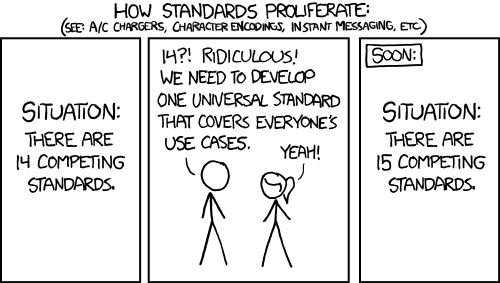
\includegraphics{./figures/xkcdstandards.png}
\caption{XKCD cartoon \#927.}\label{fig:xkcd}
}
\end{figure}

You can never cover all use cases, as is the goal of the character in
fig.~\ref{fig:xkcd}. In the future, ecological data will be used and
combined in ways we cannot anticipate in the present. To avoid the ``15
standards'' in fig.~\ref{fig:xkcd}, standards must be \emph{extendable},
such that building onto an existing standard is always easier than
building a new one, while not altering the behavior of the original
standard.

The geospatial communit alleviated the 15-standards problem issue with
the Geospatial Data Abstraction Libary (GDAL; GDAL/OGR contributors
2021), a software library for interfacing with different formats of
geospatial data. This enabled conversion between a large number of
legacy data types and the GDAL preferred format, \texttt{GeoTIFF}, and
in part led to \texttt{GeoTIFF}'s increasing ubiquity. Using software to
define ``living standards'' (a la GDAL) enables this extendability, and
makes standards more flexible, and is best enabled when the evolution of
a standard is democratic and open source.

What is to be learned from the history of data standardization? The
primary take-aways are that good standards are unambiguous, open and
free to implement, extendable, and able to change over time without
breaking backward compatibility. Standards tend to become widely adopted
with the support of institutions (e.g.~FASTA and NCBI, FITS and NASA),
which can be enabled by requiring data available in standardized format
prior to publication (e.g.~FASTA sequences made available on GenBank for
most genomics journals).

\hypertarget{using-julia-to-define-living-data-standards}{%
\section{\texorpdfstring{Using \texttt{Julia} to define living data
standards}{Using Julia to define living data standards}}\label{using-julia-to-define-living-data-standards}}

Why has standardization proven difficult in ecology? The are no fixed
set of variables used in ecological studies, and there are good reasons
to use different formats to represent the same data depending on the
context in which that data is used. The Ecological Metadata Langauge
(EML) format has been proposed (Jones et al. 2019) to solve this
problem, yet for the reasons explored in the previous section,
standardization through file-format faces challenges when faced data
that is highly variable in form and format, as is the case in
macroecology.

Here we propose defining a living standard for ecological data within
the \texttt{Julia} programming language. \texttt{Julia} adopts design
patterns from object-oriented languages, and enables building
hierarchies of abstract and concrete types without the heavyhanded type
syntax of lower level objected-oriented languages. How do we define a
standard using this type system? Each distinct category of information
(e.g.~location, species, environmental variables, and so on) has a
corresponding abstract type (e.g.~\texttt{AbstractLocation},
\texttt{AbstractSpecies}, \texttt{AbstractEnvironmentalVariable}). Then,
we define concrete types for each of the different ways you can
represent a given category of information (fig.~\ref{fig:concept}).

\begin{figure}
\hypertarget{fig:concept}{%
\centering
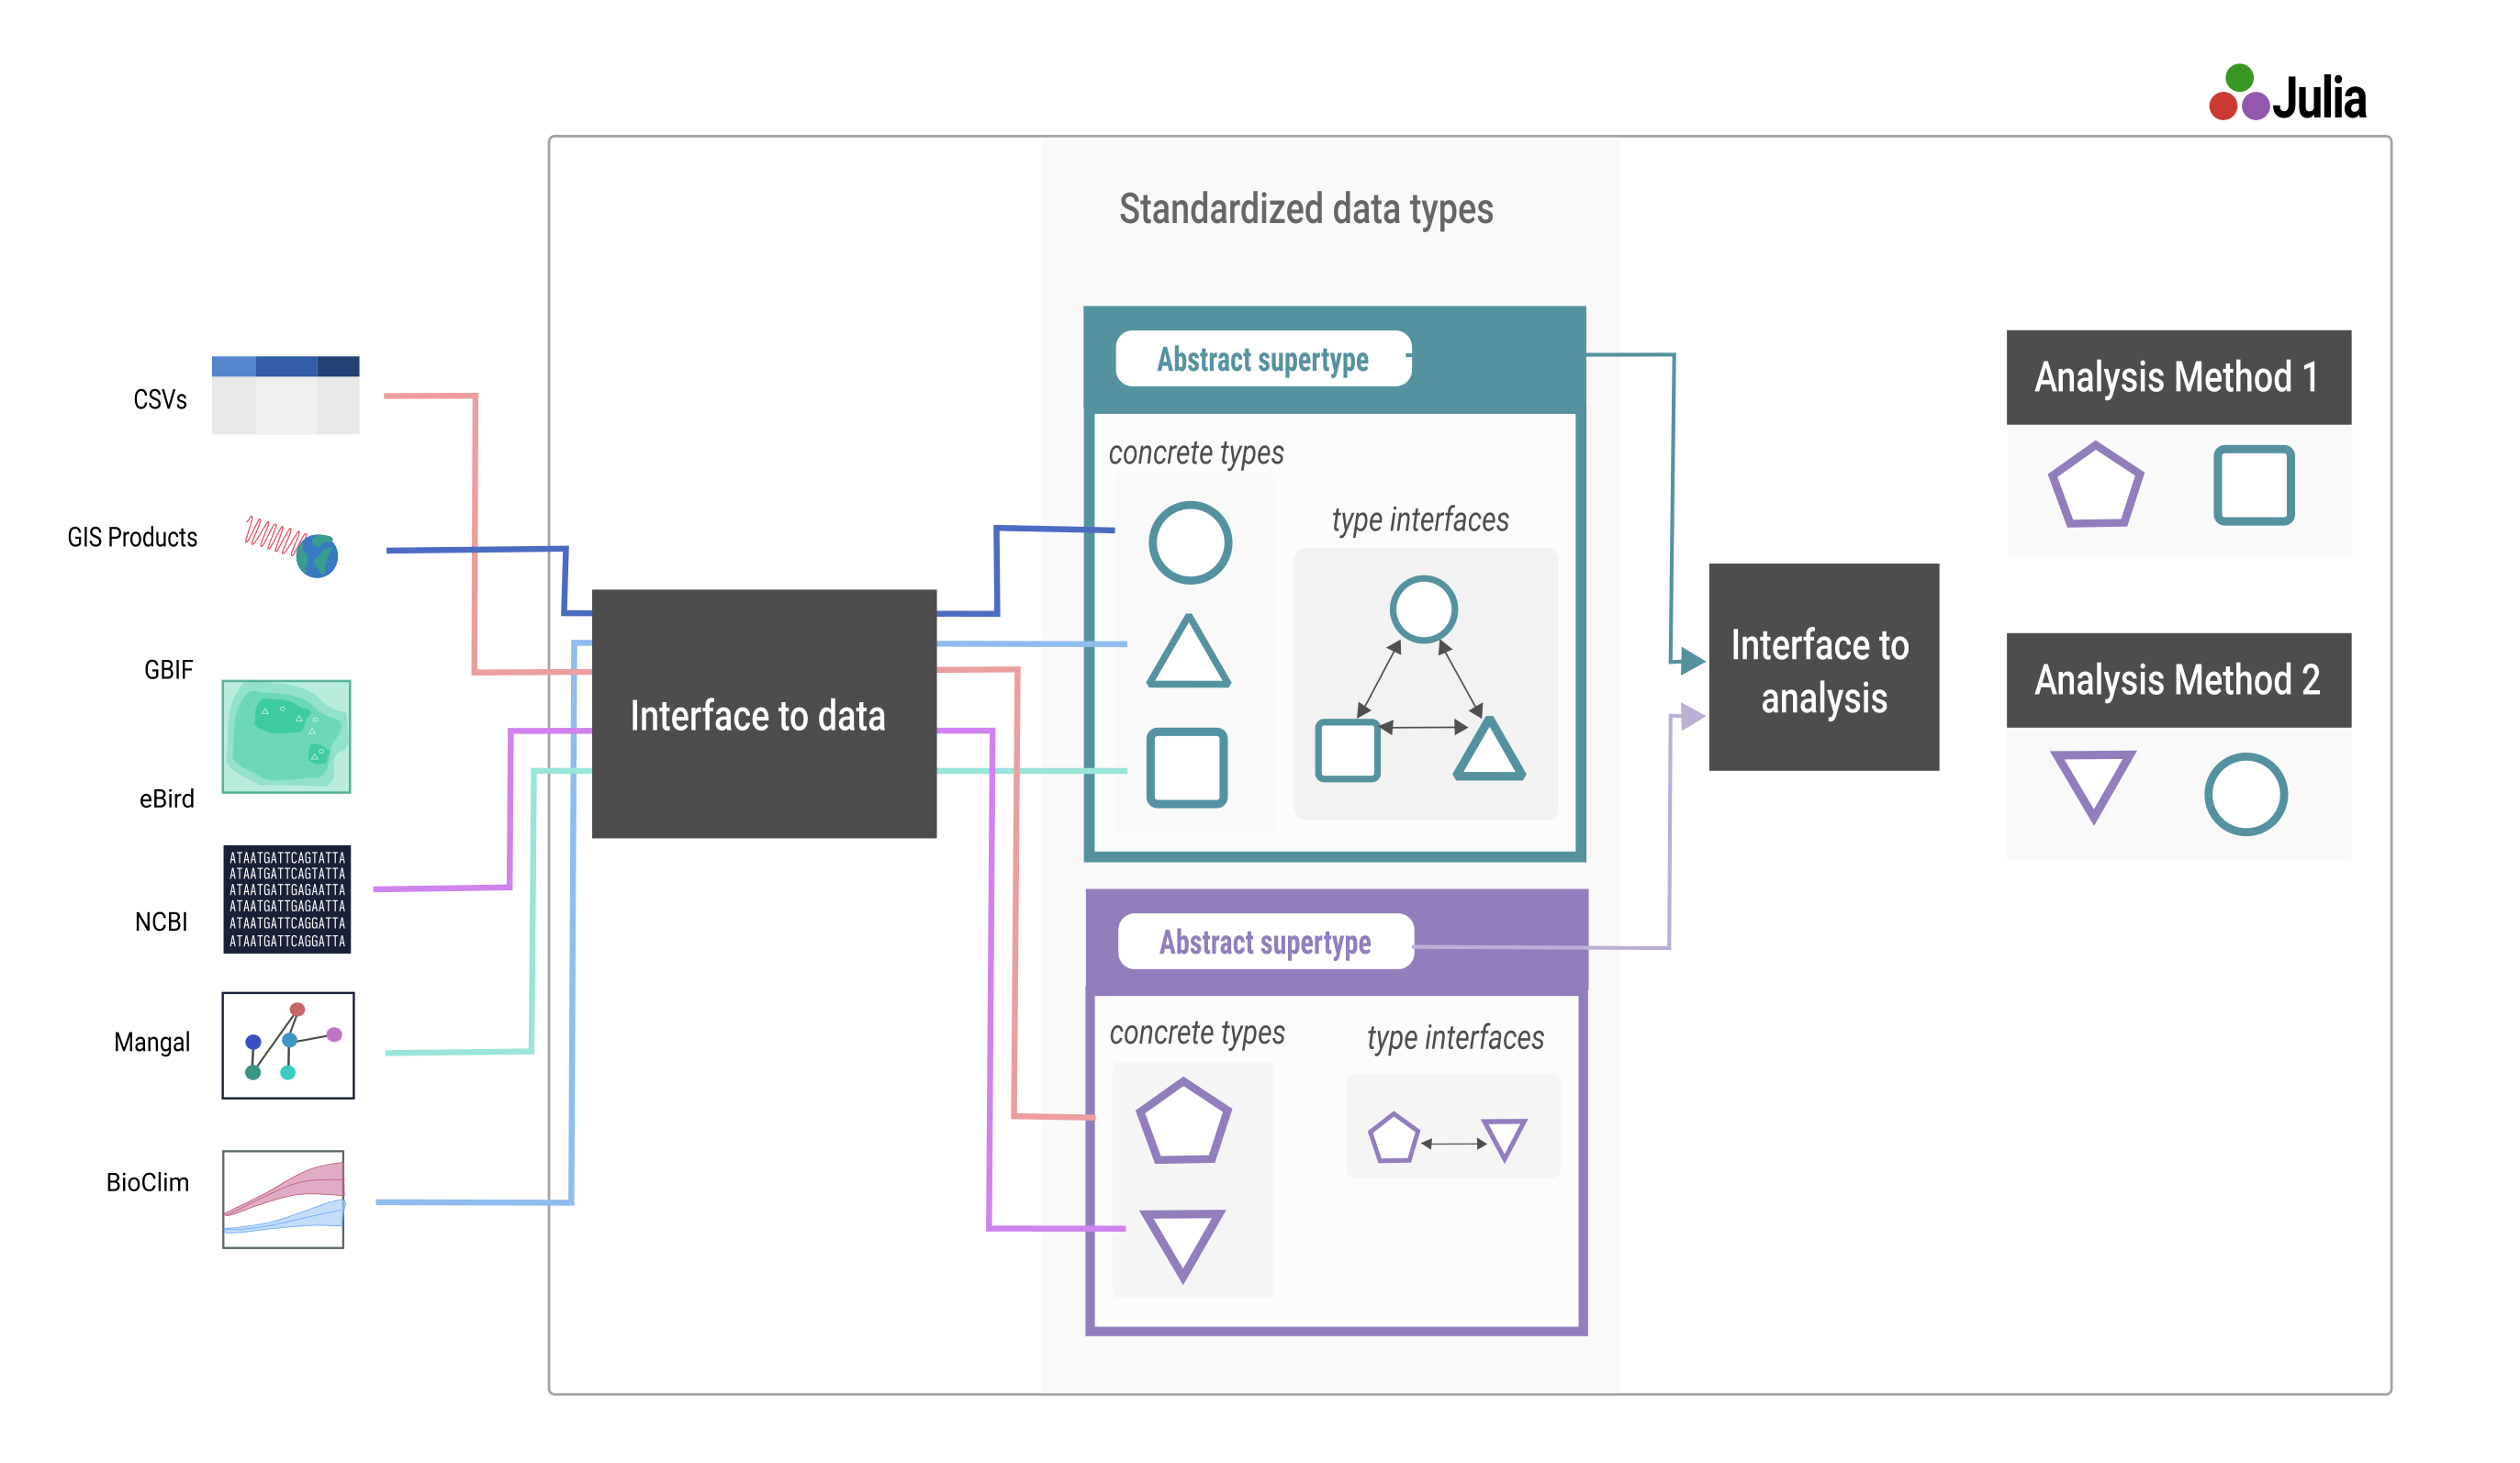
\includegraphics{./figures/concept.png}
\caption{An illustration of how the Julia type system enables
standardization of data while allowing for flexibility for the input
data format. Two standardized data types (purple and teal), each of
which are supertypes for specific concrete types (different shapes).
Each abstract supertype defines interfaces between its concrete types.
This means the user can pass data to analysis methods that require
specific data types in any form, and the interface to analysis converts
the data into the appropriate type.}\label{fig:concept}
}
\end{figure}

As an example, consider the increasingly ubiquitous case of attempting
to associate climate data (derived from WorldClim, CHLSEA, or similar)
with species occurrence data (Dansereau and Poisot 2021). Both
observations contain information about an \texttt{AbstractLocation}. If
the climate data is in a raster format, and the locations are in
coordinates, we could define concrete types \texttt{RasterLocation} and
\texttt{CoordinateLocation}, both of which are subtypes of
\texttt{AbstractLocation}. Some methods of analysis might want this data
in the form of \texttt{RasterLocation}s. Others might want
\texttt{CoordinateLocation}s. If we define a way to convert between
\texttt{RasterLocation} and \texttt{CoordinateLocation}, then it doesn't
matter what the original type of data is passed into the analysis
method, the ``interface to analysis'' can convert this data to the
proper type (see analysis panel of fig.~\ref{fig:concept}).

\texttt{Julia} is an ideal candidate to build this sort of standard, in
large part due to its type system. However beyond this \texttt{Julia}
serves to become the future of computing in biodiversity science. It is
a modern language designed for high-performance scientific computing
with expressive syntax that feels like writing high-level interpreted
languages (e.g.~Python, R, MATLAB) but with performance that rivals
\texttt{C}. \texttt{Julia} has built-in tools for testing, distributed
computing on CPUs and GPUs, and a package manager and ecosystem with
state-of-the art tools for data science, machine learning (Innes 2018;
Ge, Xu, and Ghahramani 2018), simulation (Harris and Reeve 2021), and
visualization.

Defining a living standard for ecological data in \texttt{Julia} will
make it easier to combine data from different sources by splitting the
process of data aggregation from the process of analysis. Integrating
data from a particular study, or a new database, would be as simple as
implementing the interface from the data source to the standardized
types. Data from individual studies could be incorporated into public
repositories containing both the raw data and the interface to Julia
data structures, and this combined data/interface package is all that is
needed to either reproduce the results or incorporate that particular
study's data into analysis. This will make combining data from multiple
sources easier, and yield benefits for the development and
implementation of novel methods, as the software for analysis becomes
separate from the software for data cleaning and aggregation.

We envision a modern set of tools for ecology in \texttt{Julia} based
around the standardized types. Far outside of ecology, the term
``ecosystem'' is used metaphorically to describe a set of software tools
that work together. We imagine multiple ``trophic-levels'' of packages
for ecological science in \texttt{Julia} based around the ``basal'' set
of standardized types --- a modular set of tools that can be chained
together create arbitrarily complex analysis pipelines. that can be
scaled to meet the needs of next-generation biodiversity monitoring.

\hypertarget{references}{%
\section*{References}\label{references}}
\addcontentsline{toc}{section}{References}

\hypertarget{refs}{}
\begin{CSLReferences}{1}{0}
\leavevmode\hypertarget{ref-Borregaard2016MorRep}{}%
Borregaard, Michael Krabbe, and Edmund M. Hart. 2016. {``Towards a More
Reproducible Ecology.''} \emph{Ecography} 39 (4): 349--53.
\url{https://doi.org/10.1111/ecog.02493}.

\leavevmode\hypertarget{ref-Dansereau2021SimJl}{}%
Dansereau, Gabriel, and Timothée Poisot. 2021. {``SimpleSDMLayers.jl and
GBIF.jl: A Framework for Species Distribution Modeling in Julia.''}
\emph{Journal of Open Source Software} 6 (57): 2872.
\url{https://doi.org/10.21105/joss.02872}.

\leavevmode\hypertarget{ref-GDAL}{}%
GDAL/OGR contributors. 2021. \emph{GDAL/OGR Geospatial Data Abstraction
Software Library}. Open Source Geospatial Foundation.
\url{https://gdal.org}.

\leavevmode\hypertarget{ref-Turing}{}%
Ge, Hong, Kai Xu, and Zoubin Ghahramani. 2018. {``Turing: A Language for
Flexible Probabilistic Inference.''} In \emph{International Conference
on Artificial Intelligence and Statistics, AISTATS 2018, 9-11 April
2018, Playa Blanca, Lanzarote, Canary Islands, Spain}, 1682--90.
\url{http://proceedings.mlr.press/v84/ge18b.html}.

\leavevmode\hypertarget{ref-Giron-Nava2017QuaArg}{}%
Giron-Nava, A, Cc James, Af Johnson, D Dannecker, B Kolody, A Lee, M
Nagarkar, et al. 2017. {``Quantitative Argument for Long-Term Ecological
Monitoring.''} \emph{Marine Ecology Progress Series} 572 (May): 269--74.
\url{https://doi.org/10.3354/meps12149}.

\leavevmode\hypertarget{ref-Gonzalez2015ActSta}{}%
Gonzalez, Andrew, and Pedro R. Peres-Neto. 2015. {``Act to Staunch Loss
of Research Data.''} \emph{Nature} 520 (7548): 436--36.
\url{https://doi.org/10.1038/520436c}.

\leavevmode\hypertarget{ref-Harris2021EcoJl}{}%
Harris, Claire, and Richard Reeve. 2021. {``EcoSISTEM.jl - Ecosystem
Simulation Through Integrated Species-Trait Environment Modelling.''}
Zenodo. \url{https://doi.org/10.5281/zenodo.4716816}.

\leavevmode\hypertarget{ref-Heberling2021DatInt}{}%
Heberling, J. Mason, Joseph T. Miller, Daniel Noesgaard, Scott B.
Weingart, and Dmitry Schigel. 2021. {``Data Integration Enables Global
Biodiversity Synthesis.''} \emph{Proceedings of the National Academy of
Sciences} 118 (6). \url{https://doi.org/10.1073/pnas.2018093118}.

\leavevmode\hypertarget{ref-Innes2018FluEle}{}%
Innes, Mike. 2018. {``Flux: Elegant Machine Learning with Julia.''}
\emph{Journal of Open Source Software} 3 (25): 602.
\url{https://doi.org/10.21105/joss.00602}.

\leavevmode\hypertarget{ref-Jones2019EcoMet}{}%
Jones, Matthew, Margaret O'Brien, Bryce Mecum, Carl Boettiger, Mark
Schildhauer, Mitchell Maier, Timothy Whiteaker, Stevan Earl, and Steven
Chong. 2019. {``Ecological Metadata Language Version 2.2.0.''} KNB Data
Repository. \url{https://doi.org/10.5063/F11834T2}.

\leavevmode\hypertarget{ref-Kahn2011FutGen}{}%
Kahn, S. D. 2011. {``On the Future of Genomic Data.''} \emph{Science}
331 (6018): 728--29. \url{https://doi.org/10.1126/science.1197891}.

\leavevmode\hypertarget{ref-Kuhl2020EffBio}{}%
Kühl, Hjalmar S., Diana E. Bowler, Lukas Bösch, Helge Bruelheide, Jens
Dauber, David. Eichenberg, Nico Eisenhauer, et al. 2020. {``Effective
Biodiversity Monitoring Needs a Culture of Integration.''} \emph{One
Earth} 3 (4): 462--74.
\url{https://doi.org/10.1016/j.oneear.2020.09.010}.

\leavevmode\hypertarget{ref-Poisot2019EcoDat}{}%
Poisot, Timothée, Anne Bruneau, Andrew Gonzalez, Dominique Gravel, and
Pedro Peres-Neto. 2019. {``Ecological Data Should Not Be So Hard to Find
and Reuse.''} \emph{Trends in Ecology \& Evolution} 34 (6): 494--96.
\url{https://doi.org/10.1016/j.tree.2019.04.005}.

\leavevmode\hypertarget{ref-Zimmerman2008NewKno}{}%
Zimmerman, Ann S. 2008. {``New Knowledge from Old Data: The Role of
Standards in the Sharing and Reuse of Ecological Data.''} \emph{Science,
Technology, \& Human Values} 33 (5): 631--52.
\url{https://doi.org/10.1177/0162243907306704}.

\end{CSLReferences}

\end{document}
